\documentclass[tikz,border=3pt]{standalone}
\usepackage[T1]{fontenc}
\usepackage[sfdefault]{FiraSans}
\usepackage{newtxsf}
\usepackage{pgfplots}
\usepackage[eulergreek]{sansmath}
\pgfplotsset{compat=1.11}
% % % % % % % % % % % % % % % % % % %DEFINITIONS MINE
\newcommand\mlex{M^{\scriptscriptstyle L}}
\newcommand\msyn{M^{\scriptscriptstyle S}}
\newcommand\mstd{M^{\scriptscriptstyle T}}
\newcommand\slex{S^{\scriptscriptstyle L}}
\newcommand\ssyn{S^{\scriptscriptstyle S}}
\newcommand\sstd{S^{\scriptscriptstyle T}}


\begin{document}
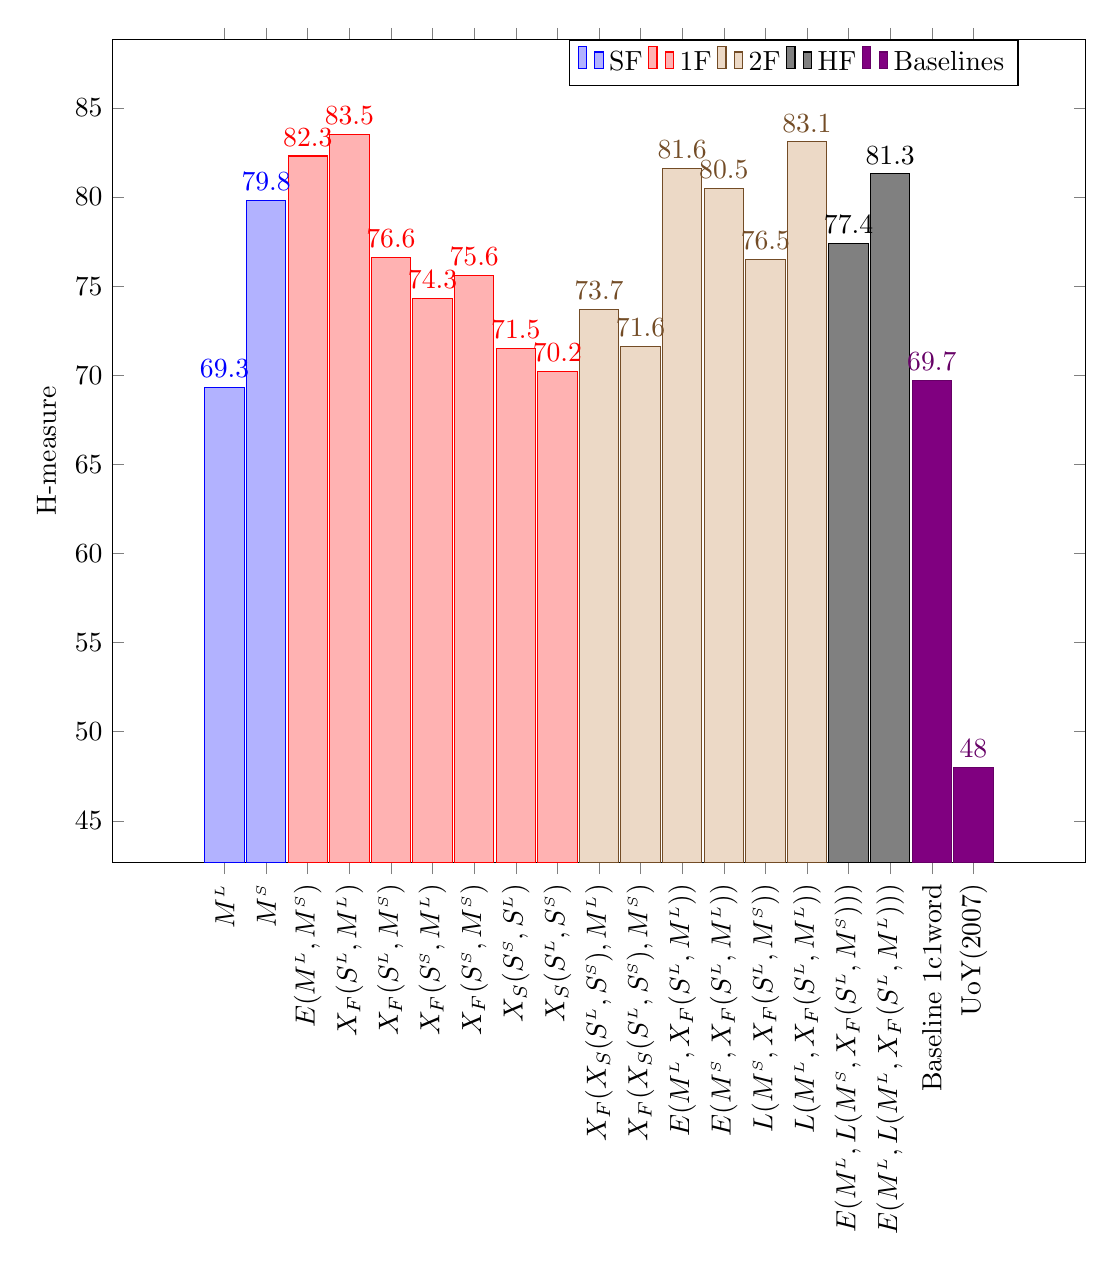
\begin{tikzpicture}
\pgfplotsset{compat=1.8}
\begin{axis}[
%	xtick distance={160},
    ybar=-0.5cm,
    width=1.15\linewidth,
    enlargelimits=0.15,
    domain = 0:90,
    xmin=0, xmax=90,
%    x=1mm, % Distance between the centers of the bars
%    enlarge x limits={abs=1cm}, % The distance between the center of the first bar and the left edge
%    enlarge y limits=false,
    legend style={at={(0.7,1)},anchor=north,legend columns=-1},
    ylabel={H-measure},
%    xmin=0, xmax=85,
    xticklabels={
	    {$\mlex$},
	    {$\msyn$},
	    {$E(\mlex, \msyn)$},
	    {$X_F(\slex, \mlex)$},
	    {$X_F(\slex, \msyn)$},
	    {$X_F(\ssyn, \mlex)$},
	    {$X_F(\ssyn, \msyn)$},
	    {$X_S(\ssyn, \slex)$},
	    {$X_S(\slex, \ssyn)$},
	    {$X_F(X_S(\slex, \ssyn), \mlex)$},
	    {$X_F(X_S(\slex, \ssyn), \msyn)$},
	    {$E(\mlex, X_F(\slex, \mlex))$},
	    {$E(\msyn, X_F(\slex, \mlex))$},
	    {$L(\msyn, X_F(\slex, \msyn))$},
	    {$L(\mlex, X_F(\slex, \mlex))$},
	    {$E(\mlex, L(\msyn, X_F(\slex, \msyn)))$},
	    {$E(\mlex, L(\mlex, X_F(\slex, \mlex)))$},
	    Baseline 1c1word,
	    UoY(2007)
    },
    xtick={0,5,...,90},
    nodes near coords,
    nodes near coords align={vertical},
    x tick label style={rotate=90,anchor=east},
    ]
\addplot+[mark=none, bar width=.5cm]  coordinates {(0,69.3) (5,79.8)};
\addplot+[mark=none, bar width=.5cm]  coordinates {(10,82.3) (15,83.5) (20,76.6) (25,74.3) (30,75.6) (35,71.5) (40,70.2)};
\addplot+[mark=none, bar width=.5cm]  coordinates {(45,73.7) (50,71.6) (55,81.6) (60,80.5) (65,76.5) (70,83.1)};
\addplot+[mark=none, bar width=.5cm]  coordinates {(75,77.4) (80,81.3)};
\addplot+[mark=none, bar width=.5cm]  coordinates {(85,69.7) (90,48.0)};

\legend{SF,1F,2F,HF, Baselines}
\end{axis}
\end{tikzpicture}
\end{document}